\section{Approach}
\label{sec-cl2017:approach}

\begin{figure}[t!]
\centering

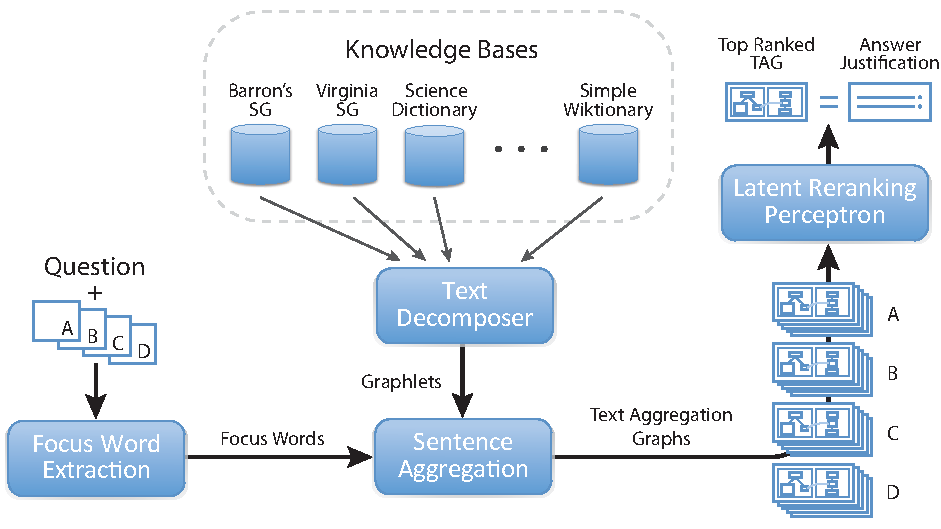
\includegraphics[width=1.0\textwidth]{mainmatter/tacl2015-tig/tag_architecture6c.pdf}

%space{-2mm}
\caption{Our QA approach, which centers on the construction of answer justifications as text aggregation graphs, and ranking them using a model that treats the justification quality as a latent variable.}
%space{-2mm}
\label{fig:architecture}
%\end{center}
\end{figure}

The architecture of our proposed QA approach is illustrated in Figure~\ref{fig:architecture}, and proceeds in a stage-like fashion.  

Prior to the QA task, in an offline process, we decompose sentences from six corpora into a lightly-structured graphical representation ("graphlets") that splits sentences on clausal and prepositional boundaries (Section~\ref{sec-cl2017:tag}). As shown later, this is fundamental to the creation and evaluation of answer justifications.  All other stages of the framework occur online. 

The QA pipeline receives as input questions with multiple choice answers, similar to the questions shown in Table~\ref{tab:inferenceexamples}, and proceeds as follows. First, the questions are fed into a focus word extractor (Section \ref{sec-cl2017:focuswords}) that produces a weighted list of the keywords from both the question and answer candidates, sorted in descending order of their likely relevance to the information needed in the question. These keywords are used by the sentence aggregation component (Section \ref{sec-cl2017:tag}) to create an exhaustive list of potential answer justifications, for each answer candidate.  These answer justifications are in the form of text aggregation graphs (TAGs), each composed of two to three graphlets produced by the above preprocessing step.

After the sentence aggregation step, each of the multiple choice answers has a long list of candidate justifications.  Because of the large number of candidate justifications created for each question/answer pair (typically tens or hundreds of thousands), we filter the list to include only the top $k$ justifications based on an inexpensive score, implemented as the sum of the weights of the focus words present in each justification\footnote{We keep ties in this filtered list, which, due to the simplicity of the score, may increase the size of the filtered lists considerably. For example, if $k=25$, it is common that the filtered list includes between $100$ and $1,000$ candidate justifications.}. 
Using the focus words, we extract a number of features from each candidate justification that measure how well the justification answers the question (Section ~\ref{sec-cl2017:scoring}), and present this information to a latent-variable perceptron ranker (Section~\ref{sec-cl2017:perceptron}).  This learning framework learns which answer candidate is correct based on the candidate justifications, while also jointly learning to rank justification quality as a latent variable, selectively elevating good answer justifications to the top of the list.  

The candidate answer with the highest-scoring justification is taken to be the correct answer.  While the justification is expressed in the form of a text aggregation graph to make it easier to assemble and evaluate, we use the original sentences from the knowledge base used to construct that text aggregation graph as a human-readable justification for why that answer candidate is correct. 
